\documentclass[a4paper,oneside,10pt]{article}
\usepackage{wallpaper}
\usepackage{float}
\usepackage[utf8]{inputenc}
\usepackage{circuitikz}
\usepackage{listings}
\usepackage{indentfirst}
\lstdefinelanguage{Arduino}{
	language=C++,
	morekeywords={
		void,
		setup,
		loop,
		pinMode,
		analogRead,
		delay,
		map,
		constrain,
		Serial,
		Wire,
		HIGH,
		LOW,
		INPUT,
		OUTPUT
	},
	morekeywords=[2]{
		Servo,
		Adafruit_ADS1115,
		begin,
		attach,
		write,
		print,
		println,
		readADC_SingleEnded,
		setGain
	},
	sensitive=true
}
\lstdefinestyle{mystyle}{
	columns=fullflexible,
	frame=single,
	breaklines=true,
	numbers=left,
	tabsize=2,
	belowcaptionskip=1\baselineskip,
	language=Arduino,
	showstringspaces=false,
	basicstyle=\footnotesize\ttfamily,
	keywordstyle=\bfseries\color{green!40!black},
	commentstyle=\itshape\color{purple!40!black},
	identifierstyle=\color{blue},
	stringstyle=\color{orange},
	keywordstyle=[2]\bfseries\color{green!40!black},
	literate=
	{á}{{\'a}}1
	{é}{{\'e}}1
	{í}{{\'i}}1
	{ó}{{\'o}}1
	{ú}{{\'u}}1
	{à}{{\`a}}1
	{â}{{\^a}}1
	{ê}{{\^e}}1
	{ô}{{\^o}}1
	{ã}{{\~a}}1
	{õ}{{\~o}}1
	{ç}{{\c{c}}}1
	{Á}{{\'A}}1
	{É}{{\'E}}1
	{Í}{{\'I}}1
	{Ó}{{\'O}}1
	{Ú}{{\'U}}1
	{À}{{\`A}}1
	{Â}{{\^A}}1
	{Ê}{{\^E}}1
	{Ô}{{\^O}}1
	{Ã}{{\~A}}1
	{Õ}{{\~O}}1
	{Ç}{{\c{C}}}1
}
\lstset{style=mystyle}
\renewcommand{\lstlistingname}{Código}
\usepackage{graphicx}
\usepackage[alf]{abntex2cite}
\usepackage{url}
\usepackage{hyphenat}
\usepackage[brazil]{babel}
\setlength{\textwidth}{16cm} %
\setlength{\textheight}{23cm} %
\setlength{\oddsidemargin}{0cm} %
\setlength{\evensidemargin}{0cm} %
\setlength{\topmargin}{0cm}
\CenterWallPaper{1.01}{bg.pdf}

\begin{document}

\noindent Relatório 7: Sensores e atuadores. \\
Internet das Coisas - Integral\\
Prof. Gabriel de Freitas Fernandes\\
2026.2\\
\\
\textbf{EQUIPE:} \\ Arthur Peixoto - 170.214 \\ Gabriel Oliva Gurgel - 168.860 \\ Guilherme Samuel dos Santos - 168.867

\section{Introdução}
Um dos usos mais comuns relacionados aos sistemas embarcados é a aquisição de grandezas físicas (no mundo real) por meio de sensores e o uso dessas informações para o acionamento de atuadores. Nesse contexto, o microcontrolador atua como elemento central, responsável por converter sinais do ambiente em dados digitais e, a partir deles, gerar sinais de controle adequados para o dispositivo que se deseja acionar.

Nesta prática, será realizada uma atividade envolvendo um ESP32, um sensor de luminosidade do tipo \textit{Light Dependent Resistor} (\textbf{LDR}) e um servomotor \textbf{MG996R}. Em um primeiro modelo, o ESP32 realizará a leitura do LDR por meio de seu conversor analógico-digital (ADC) interno e converterá o valor adquirido em um sinal de controle da posição angular do servomotor. Dessa forma, a posição do servo passa a variar em função da intensidade luminosa incidente sobre o sensor.

Em um segundo momento, o modelo inicial será aprimorado com a inclusão do módulo conversor analógico-digital externo \textbf{ADS1115} (com melhor resolução) que se comunica com o microcontrolador por meio do protocolo I2C. A substituição do ADC interno do ESP32 por esse módulo visa melhorar a resolução, a linearidade e a estabilidade das medições, uma vez que o conversor nativo do ESP32 apresenta não linearidades e maior sensibilidade a ruído. Essa etapa permite, ainda, a comparação direta entre as duas abordagens de aquisição e a análise de seu impacto na qualidade do controle do motor.

\section{Prática}

\subsection{ADC interno}
O ESP32 dispõe de dois conversores analógico-digitais de aproximação sucessiva (SAR) de 12 bits, denominados \textbf{ADC1} e \textbf{ADC2}, segundo a sua documentação oficial \cite{espressifESP32}. O ADC1 possui oito canais, distribuídos nos pinos GPIO32 a GPIO39, enquanto o ADC2 possui dez canais, mas compartilha recursos com o módulo Wi-Fi e, por isso, tem seu uso restringido quando este está ativo. Para a realização da prática, foi adotado o \textbf{ADC1}. Não foi necessário testar outra maneira de ligação.

\subsection{ADC externo e comunicação I2C}
Embora o ESP32 possua conversores analógico-digitais internos, sua curva de resposta apresenta não linearidades e variações ao longo da faixa de medição. Além disso, o ruído gerado pelos módulos de rádio (por exemplo, Wi-Fi e \textit{Bluetooth Low Energy}) pode se acoplar às leituras, de modo que o uso direto do ADC interno não é recomendável quando se deseja maior precisão. Uma alternativa usada pela comunidade em fóruns é empregar um conversor externo, como o \textbf{ADS1115}, conectado ao microcontrolador por meio do protocolo I2C.
O ESP32 dispõe de dois controladores I2C, denominados \textbf{I2C0} e \textbf{I2C1}, segundo a sua documentação pela EspressIf. Para a realização da prática, foi adotada a interface \textbf{I2C0}, utilizada por padrão pela biblioteca \texttt{Wire}, com o pino \textbf{GPIO21} como linha de dados (SDA) e o pino \textbf{GPIO22} como linha de relógio (SCL). Essa foi a configuração inicialmente definida pelo grupo, e o módulo \textbf{ADS1115} foi endereçado em \texttt{0x48}, endereço padrão obtido com o pino ADDR ligado ao GND \cite{tiADS1115}. Assim como na primeira parte da prática, não foi necessário testar outra maneira de ligação.

\subsection{Montagem Experimental}

\begin{figure}[H]
	\centering
	\begin{minipage}[b]{0.6\textwidth}
		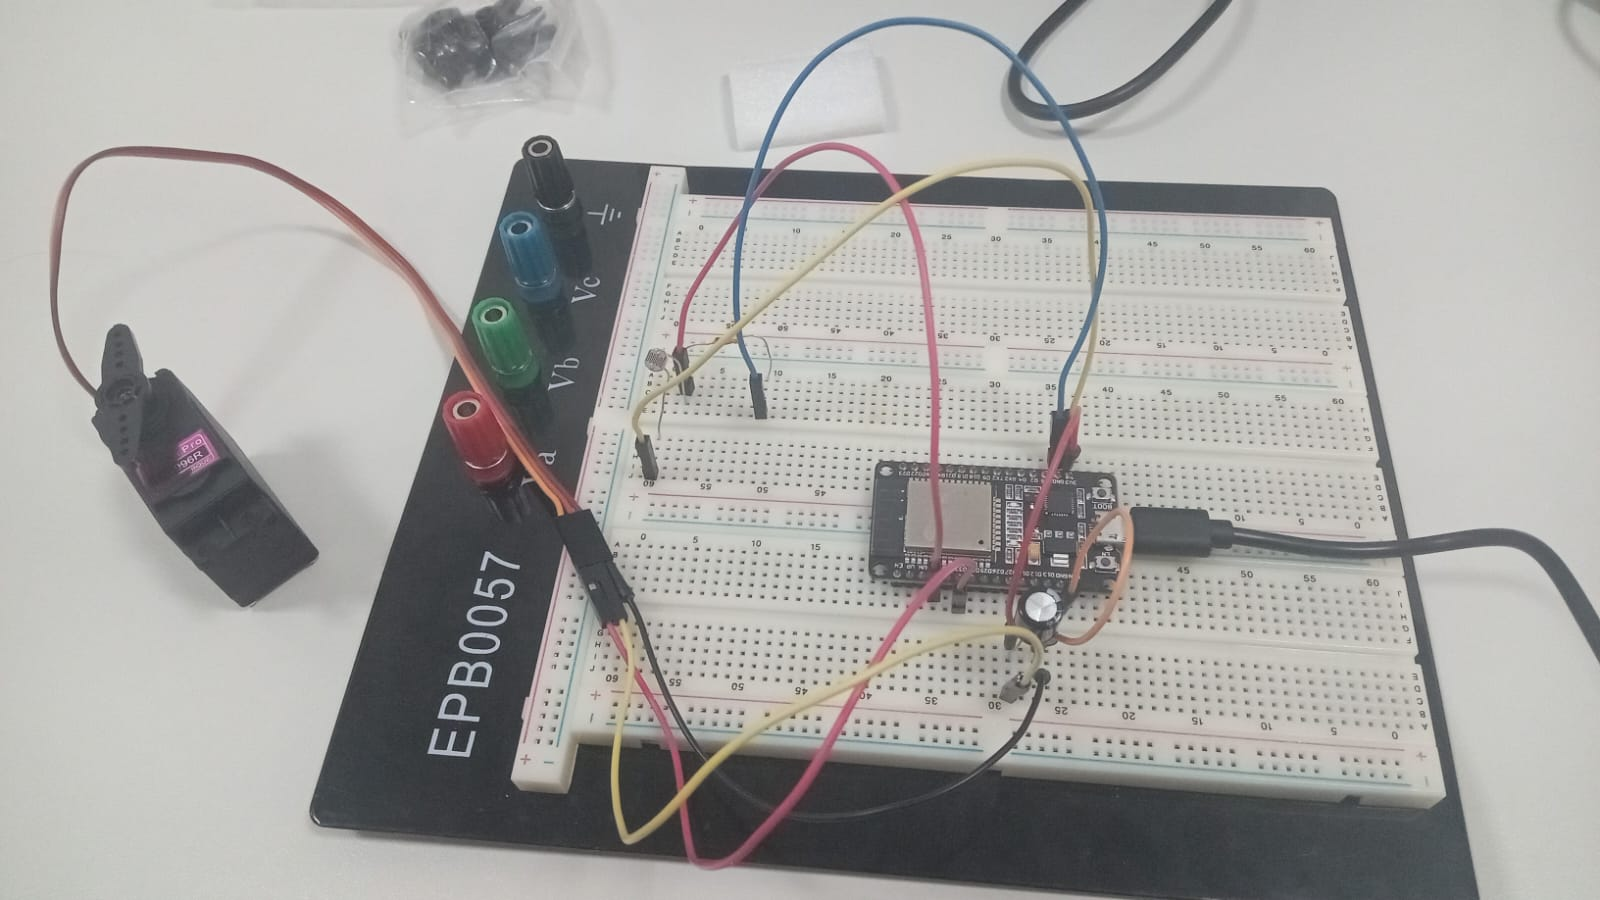
\includegraphics[width=\textwidth]{v1}
		\caption{Usando ADC interno}
	\end{minipage}
	\hfill
\end{figure}
\begin{figure}[H]
	\centering
	\begin{minipage}[b]{0.4\textwidth}
	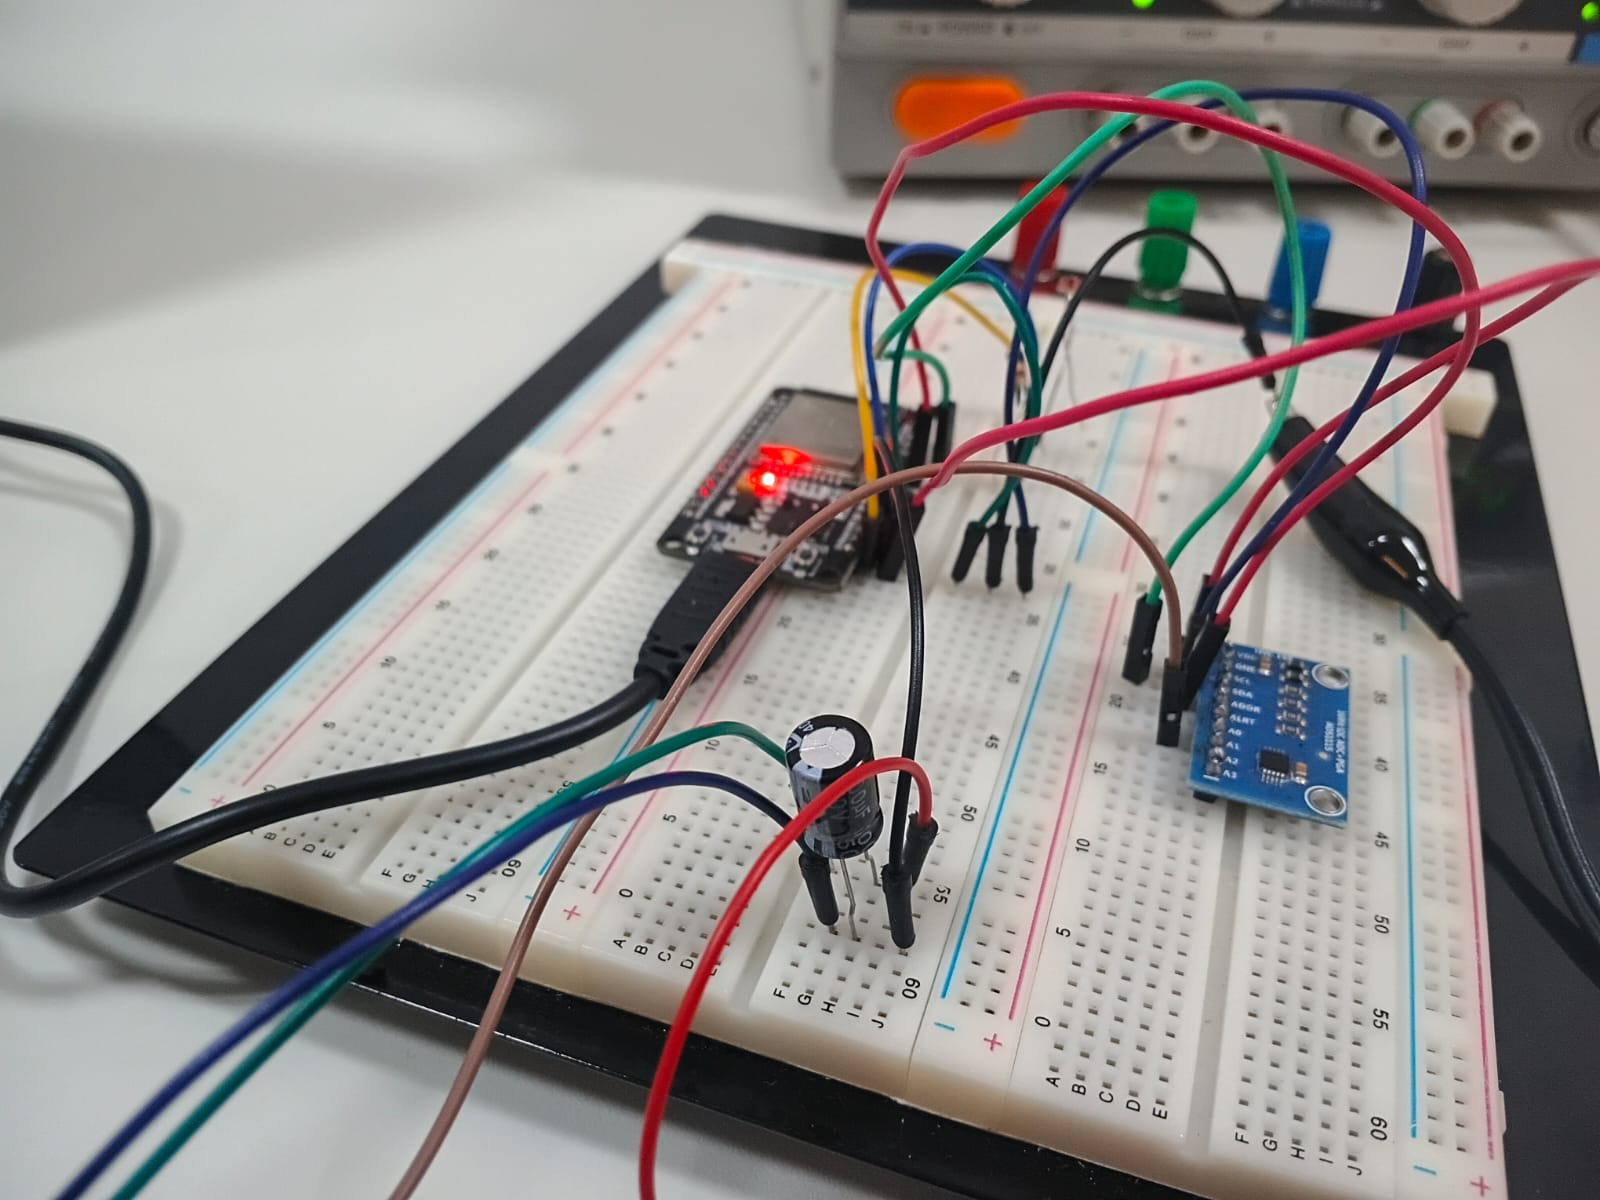
\includegraphics[width=\textwidth]{v2}
	\caption{Usando ADC externo}
	\end{minipage}
	\hfill
\end{figure}

\subsection{Código}

Para a leitura do sensor, um dos pinos foi configurado como entrada por meio da função \texttt{pinMode}, por pertencer ao \textbf{ADC1} e ser um pino exclusivo de entrada. A função \texttt{analogRead} retorna um valor inteiro de 12 bits, ou seja, na faixa teórica de 0 a 4095. Esse valor foi mapeado linearmente para a faixa de 0° a 180° por meio da função \texttt{map}, utilizando 4095 como limite superior da entrada. Vale a pena considerar que $2^{12} = 4096$, apesar que dificilmente ele passa do valor (aproximado) de 3500.

O sinal de pulso de controle do servo \textbf{MG996R} é gerado pela biblioteca \texttt{ESP32Servo}, por meio da função \texttt{servo.write}, que recebe o ângulo desejado e o converte na largura de pulso correspondente.

O valor bruto lido pelo ADC (sensor LDR) é enviado ao Monitor Serial a cada iteração, o que permite acompanhar a variação da luminosidade e relacioná-la com a posição do servo.

\pagebreak

\lstinputlisting[caption=Versão com ADC interno]{activate_mg996r_servo_1.ino}

Para a leitura do sensor, o módulo ADS1115 foi inicializado por meio da função \texttt{ads.begin(0x48)}, dentro de um laço \texttt{while} que repete a tentativa e imprime uma mensagem de erro no Monitor Serial enquanto o módulo não é encontrado. Dessa forma, o programa apenas prossegue após a confirmação de que a comunicação I2C com o conversor foi estabelecida, pois durante o laboratório, o nosso grupo não estava com certeza se o problema era do sensor ou do conversor/protocolo. A leitura é feita pela função \texttt{readADC\_SingleEnded(0)}, que realiza uma conversão em modo \textit{single-ended} no canal A0 e retorna um valor inteiro de 16 bits com sinal (\texttt{int16\_t}).

O valor obtido foi mapeado linearmente para a faixa de 0° a 180° por meio da função \texttt{map}, mantendo-se a mesma lógica adotada com o ADC interno, assim como a atualização do ângulo do servomotor. A única diferença está nos limites da entrada, que passaram a ser $13000$ e $17200$, em vez de $0$ e $4095$. A escolha desses valores será justificada na seção de Resultados e Discussão. 

\lstinputlisting[caption=Versão com ADC externo]{activate_mg996r_servo_2.ino}

\subsection{Resultados e Discussão}

Conseguimos verificar a mudança. Para isso, usamos uma lanterna como fonte de luz e testamos como o ângulo e a entrada de dados influenciavam o resultado.

\begin{figure}[H]
	\centering
	\begin{minipage}[b]{0.5\textwidth}
		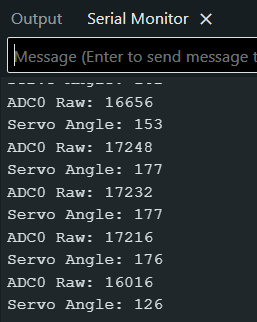
\includegraphics[width=\textwidth]{result}
		\caption{Amostra do monitoramento serial}
	\end{minipage}
	\hfill
\end{figure}

Na versão do código com o ADC externo, o valor captado pelo ADS1115 foi inicialmente exibido no Monitor Serial e, a partir das leituras observadas, os limites foram inseridos como argumentos da função \texttt{map}. Essa mudança se deve ao fato de que, com o ganho padrão da biblioteca (faixa de $\pm 6{,}144$ V, com $0{,}1875$ mV por bit), o sinal do divisor de tensão com o LDR ocupa apenas uma parte da escala de 16 bits, uma vez que o circuito foi alimentado diretamente pela saída de 3,3 V do ESP32. Não chegamos a testar o sistema com tensões de alimentação maiores.

\subsection{Verificação com Osciloscópio}

\begin{figure}[H]
	\centering
	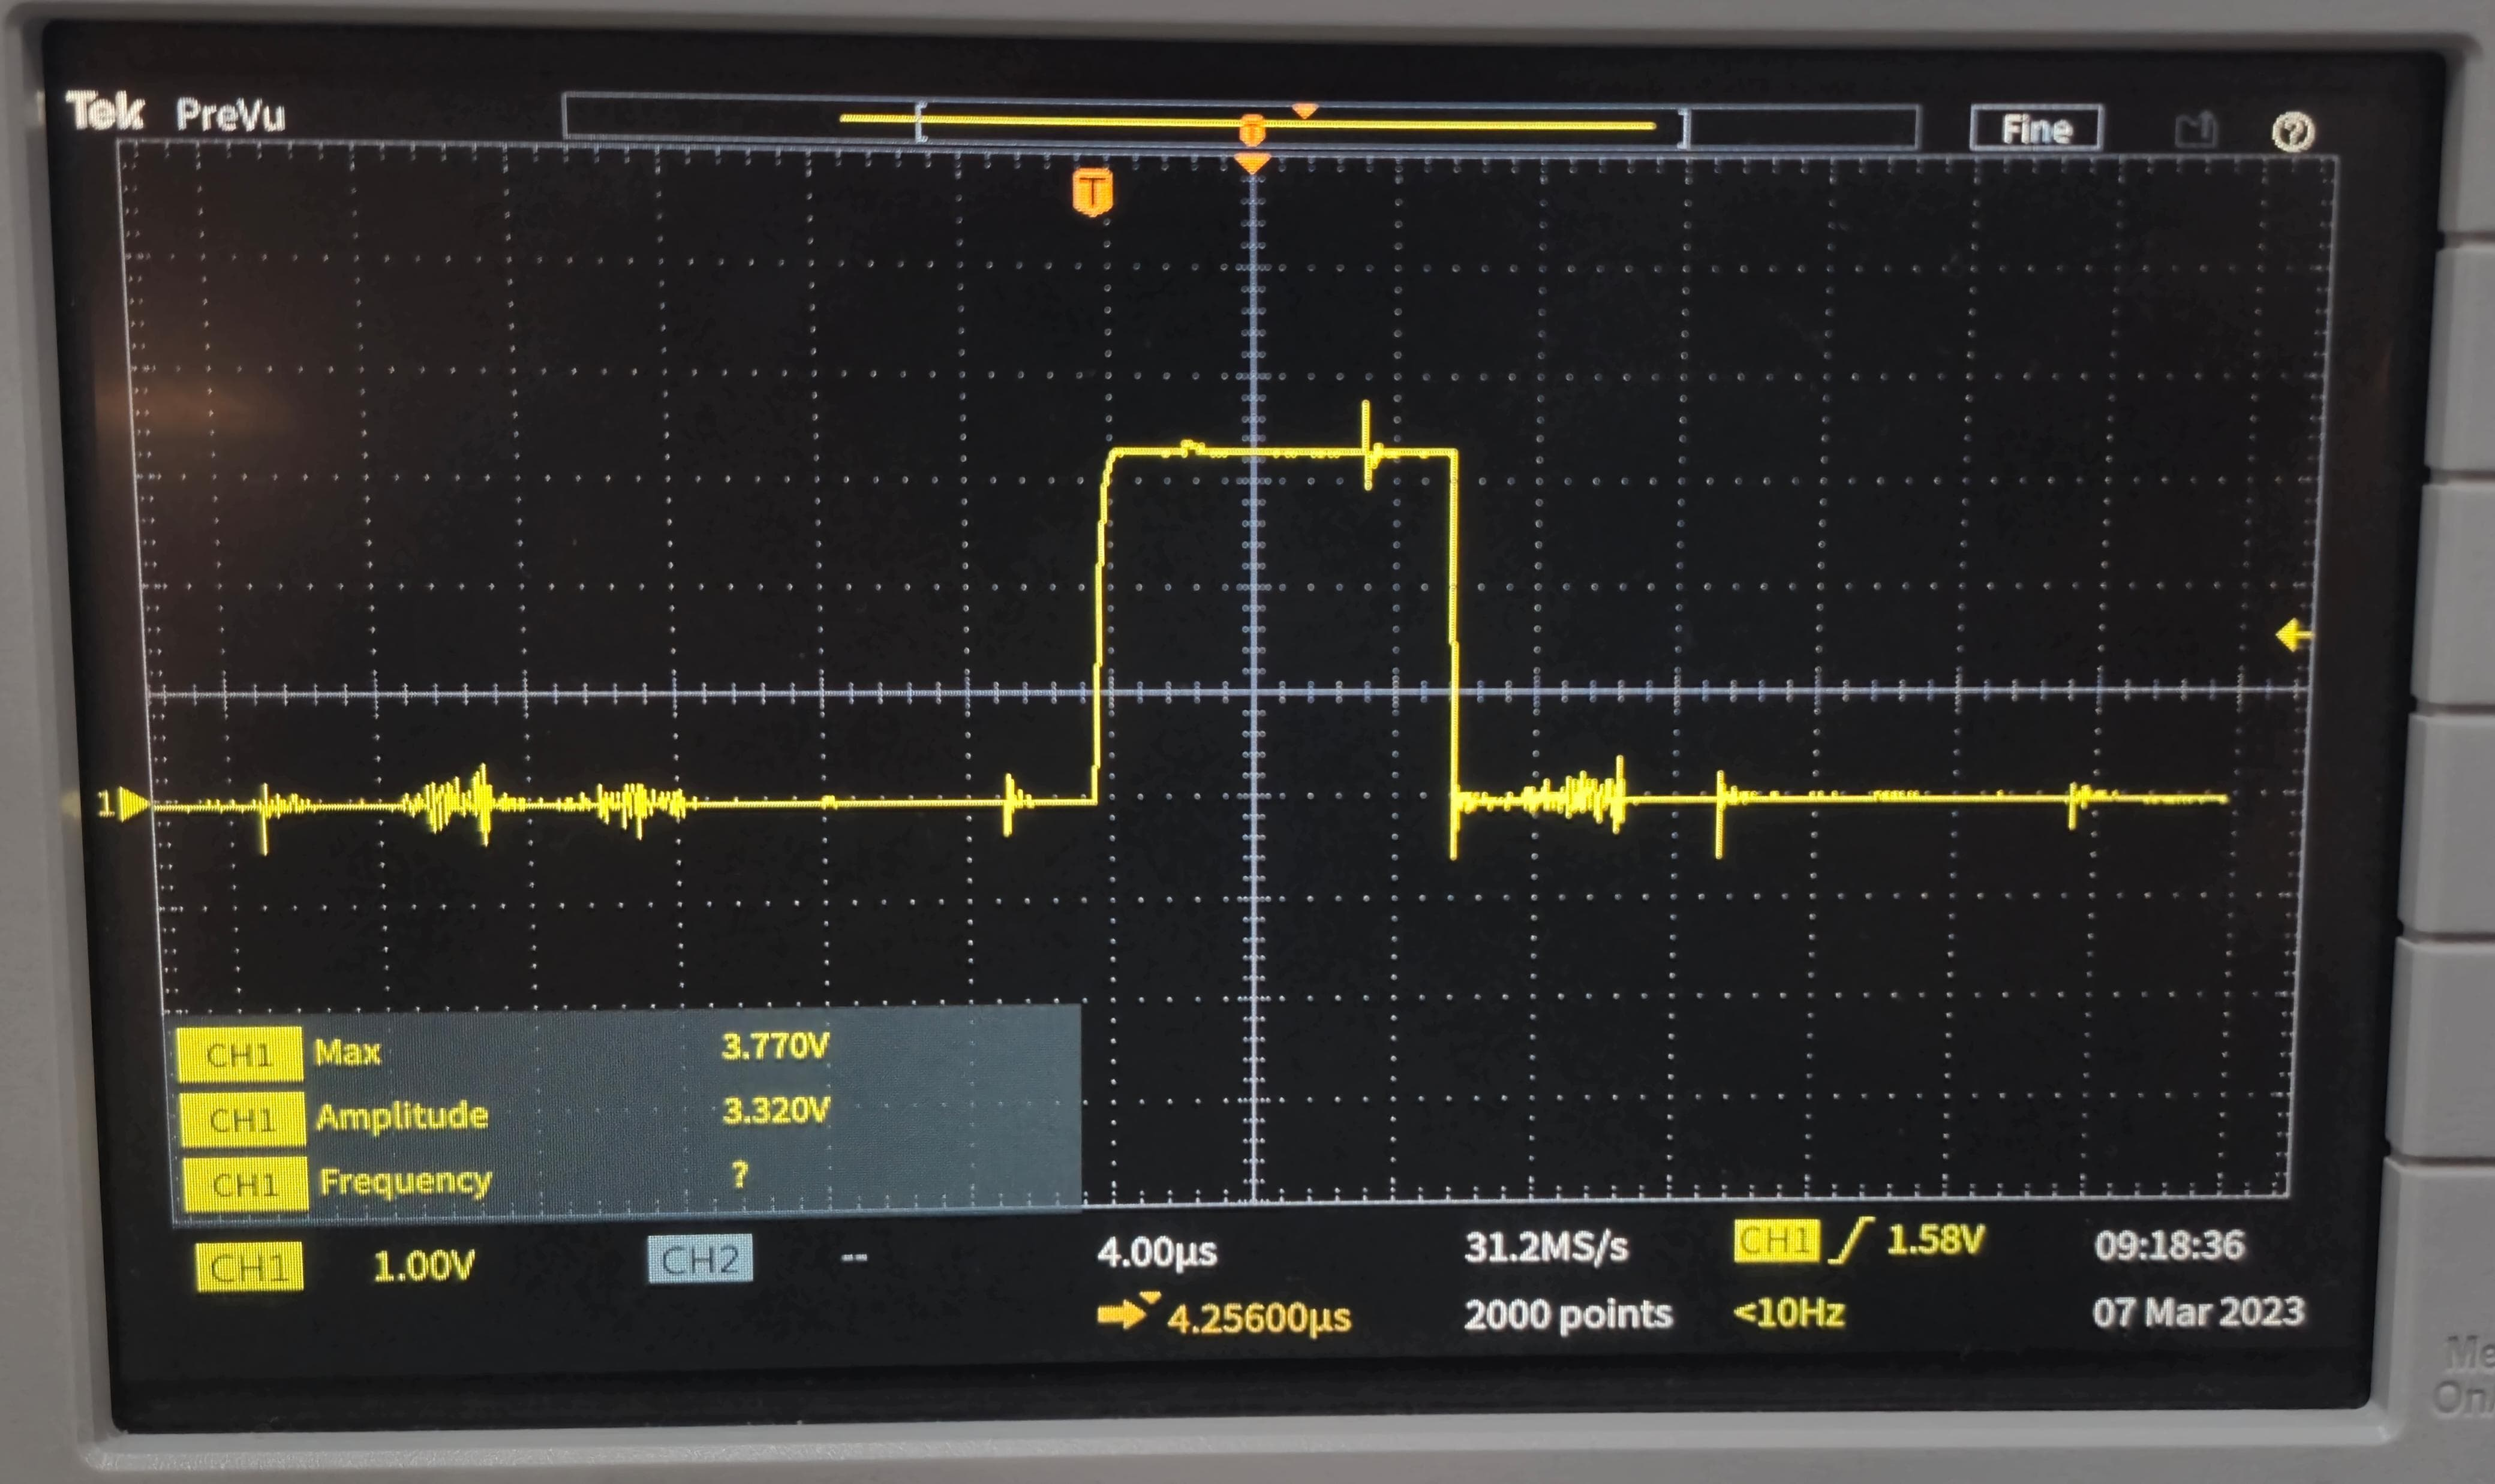
\includegraphics[scale=0.1]{oscilloscope}
	\caption{Sinal da linha SDA na comunicação entre o ADS1115 e o ESP32}
\end{figure}

Nos primeiros testes, utilizamos o osciloscópio para verificar se havia alguma interferência no sinal proveniente do LDR. Com ele, foi possível observar variações na amplitude do sinal ao regular a luminosidade incidente sobre o sensor. A Figura mostra a transmissão I2C na linha de dados (SDA), com pico em torno de 3,7 V. Como os testes foram realizados com o notebook conectado ao carregador, houve o aparecimento de ruído proveniente da fonte de energia, o que afetou as medições.

\section{Dificuldades Encontradas}

Durante a execução de ambas as partes, enfrentamos problemas para identificar corretamente a origem das falhas apresentadas pelo módulo ADS1115. Em um primeiro momento, o conversor não apresentou funcionamento adequado, e foi necessário eliminar as possíveis variáveis por exclusão. Para isso, foi realizada a observação direta das oscilações do sinal do sensor LDR, o que permitiu verificar que o sensor e o divisor de tensão operavam normalmente e que o problema estava localizado no módulo. A hipótese mais provável é a de que a falha tenha ocorrido por mau contato nas soldas dos pinos A0 e GND. Portanto, optamos por soldar uma nova unidade do ADS1115, de modo a realizar a atividade em laboratório com menos problemas de ruído, uma vez que a placa anterior acabou sendo danificada acidentalmente por um curto-circuito.

\section{Pós-Laboratório}

\subsection{Benefício de empregar um ADC externo quando o sistema contém um ESP32}
Embora o ESP32 possua conversores analógico-digitais (ADCs) internos, o uso de um componente externo como o ADS1115 traz vantagens importantes:
\begin{enumerate}
	\item \textbf{Evita conflitos com o Wi-Fi:} O segundo conversor interno do ESP32 compartilha recursos com o rádio Wi-Fi, o que pode gerar instabilidades ou bloqueios nas leituras durante o uso da rede sem fio. O ADS1115 utiliza comunicação digital ($I^2C$), operando de forma independente do Wi-Fi.
	\item \textbf{Maior precisão e linearidade:} O conversor interno do ESP32 apresenta pequenas limitações e variações de leitura em faixas muito baixas ou muito altas de tensão. O ADS1115 oferece leituras mais estáveis, lineares e confiáveis.
	\item \textbf{Maior resolução:} O ADS1115 possui resolução de 16 bits, o que permite capturar variações de sinal muito mais sutilezas do que os 12 bits nativos do ESP32.
\end{enumerate}

\subsection{Tipo de ADC empregado no ADS1115 e seu funcionamento}
O ADS1115 utiliza um conversor do tipo \textbf{Delta-Sigma ($\Delta\Sigma$)}. 

Ele funciona amostrando o sinal de entrada em uma frequência muito alta (processo conhecido como sobreamostragem) e convertendo-o em um fluxo rápido de bits. Em seguida, um filtro digital interno processa esse fluxo de dados, eliminando os ruídos de alta frequência e gerando uma leitura digital final de alta precisão e resolução na saída.

\section{Anexos}

\begin{itemize}
	\item Dois arquivos \texttt{.ino}, correspondentes as duas partes: com e sem ADC externo.
\end{itemize}

\newpage

\bibliographystyle{abntex2-alf}
\bibliography{references}
\end{document}